%!TEX root = ../BUSystematics.tex

\graphicspath{{Body/Figures/MuonLosses/}}

\section{Muon Losses}

-introduce this section better

See Sections 5.3.3 and 5.5.4 of \refref{phdthesis:2020Kinnaird} for how the lost muon term in the fits is constructed and how the associated systematic errors are estimated. In general the losses spectrum consists of triples formed using the cuts in \tabref{tab:lostmuoncuts}, and then quadruples and accidentals are subtracted for a purer sample of triples. In the case of the quadruples, the two constitutent triples are subtracted. Systematic errors are then estimated by varying the specific cuts used.


\begin{table}[h]
\centering
\setlength\tabcolsep{10pt}
\renewcommand{\arraystretch}{1.2}
\begin{tabular*}{1\linewidth}{@{\extracolsep{\fill}}lc}
  \hline
    \multicolumn{2}{c}{\textbf{Lost Muon Cuts}} \\
  \hline\hline
    Parameter & Cut \\
  \hline
    Cluster size & $\leq$ 3 crystals \\
    Cluster energy fraction & $\geq$ 0.8 in main crystal \\
    Time of flight between adjacent calorimeters & $\SI{5}{ns} \leq \Delta t_{12, 23} \leq \SI{7.5}{ns}$ \\
    Energy deposition & $\SI{100}{\MeV} \leq E_{1,2,3} \leq \SI{250}{\MeV}$ \\
    Time of flight between separated calorimeters & $\Delta t_{13} \leq \SI{14.4}{ns}$ \\
  \hline 
\end{tabular*}
\caption[Lost muon cuts]{Lost muon selection cuts. In a triple coincidence the subscripts 1, 2, and 3 correspond to the three calorimeters hit clockwise around the ring.}
\label{tab:lostmuoncuts}
\end{table}



\subsection{Cuts}

Tables \ref{tab:Tlostmuonsvariousfits} and \ref{tab:Rlostmuonsvariousfits} give the \DR's for the different datasets for different cuts used when constructing the lost muon triples spectra. The different cuts tested were including/excluding the quadruple subtraction, including/excluding the accidental subtraction, widening the time-of-flight cut, widening the energy range cut, and cutting on the low side of $\Delta t_{13}$ (in order to cut out any effects from proton or deteuron contamination which get into the triples spectrum). As shown for all cuts, the exact cuts used in the construction of the triples makes no significant difference in the final \R values. The shape of the triples spectrum is only marginally affected, the fitted \K parameter simply adjusts to compensate for any changes in statistics, and \K is weakly correlated to \R. For the systematic errors related to the time and energy cuts used in the triples spectrum, the corresponding entries for the different datasets are taken. 


There are some other entries in the combined systematics table such as the higher order coincidences, however since I subtract quadruples off I don't include such an error. I simply include the \DR in the table to give a sense of scale of the changes. Similar logic holds for the accidental subtraction cut and low side of $\Delta t_{13}$ cut, which don't correspond to specific systematic errors.



\begin{table}
\centering
\setlength\tabcolsep{10pt}
\renewcommand{\arraystretch}{1.2}
\begin{tabular*}{1\linewidth}{@{\extracolsep{\fill}}lHHHH}
  \hline
    \multicolumn{5}{c}{\textbf{T-Method $\Delta R$ with Various Lost Muon Cuts}} \\
  \hline
    Type of fit or cut & \thead{60h} & \thead{HighKick} & \thead{9d} & \thead{Endgame} \\
  \hline
    No quadruple subtraction                                & -0.2 & -0.4 & 0.1  & -0.3 \\
    No accidental subtraction                               & 0.3  & <0.1 & <0.1 & 0.2 \\
    $\SI{4}{ns} \leq \Delta t_{12, 23} \leq \SI{8.5}{ns}$   & -0.3 & <0.1 & <0.1 & <0.1 \\
    $\SI{50}{\MeV} \leq E_{1,2,3} \leq \SI{500}{\MeV}$      & 0.5  & 0.1  & 0.1  & 1.0 \\
    $\Delta t_{13} \leq \SI{12.5}{ns}$                      & -1.3 & -0.1 & 0.1  & -0.9 \\
  \hline 
\end{tabular*}
\caption[]{Effect on the fitted \R value for the T-Method fits for the Run~1 datasets with various cuts used or backgrounds subtracted. Units are in ppb.}
\label{tab:Tlostmuonsvariousfits}
\end{table}


\begin{table}
\centering
\setlength\tabcolsep{10pt}
\renewcommand{\arraystretch}{1.2}
\begin{tabular*}{1\linewidth}{@{\extracolsep{\fill}}lHHHH}
  \hline
    \multicolumn{5}{c}{\textbf{R-Method $\Delta R$ with Various Lost Muon Cuts}} \\
  \hline
    Type of fit or cut & \thead{60h} & \thead{HighKick} & \thead{9d} & \thead{Endgame} \\
  \hline
    No quadruple subtraction                                & -0.4 & 0.1  & 0.1  & -0.1 \\
    No accidental subtraction                               & <0.1 & <0.1 & -0.1 & 0.1 \\
    $\SI{4}{ns} \leq \Delta t_{12, 23} \leq \SI{8.5}{ns}$   & -0.3 & <0.1 & <0.1 & <0.1 \\
    $\SI{50}{\MeV} \leq E_{1,2,3} \leq \SI{500}{\MeV}$      & 0.3  & <0.1 & <0.1 & 0.5 \\
    $\Delta t_{13} \leq \SI{12.5}{ns}$                      & -0.8 & -0.2 & 0.1  & -0.3 \\
  \hline 
\end{tabular*}
\caption[]{Effect on the fitted \R value for the R-Method fits for the Run~1 datasets with various cuts used or backgrounds subtracted. Units are in ppb.}
\label{tab:Rlostmuonsvariousfits}
\end{table}






\subsection{Muon Loss Scale Fixed}

The R-Method is insensitive to the lost muon term in the fit and cannot converge to a value properly. I choose to include the lost muon term and fix the value of \K to that determined from a T-Method fit to the same data. The systematic error is then determined by scanning over the fixed \K value, determining the sensitivity of \R to it, and then multiplying it against the uncertainty in the \K value as determined from the T-Method fit. An example scan is shown in \figref{fig:kappaLossScan}. The results of the scans for the various datasets, and the associated systematic errors are given in \tabref{tab:systematicError_kappaLoss}.



\begin{figure}
    \centering
    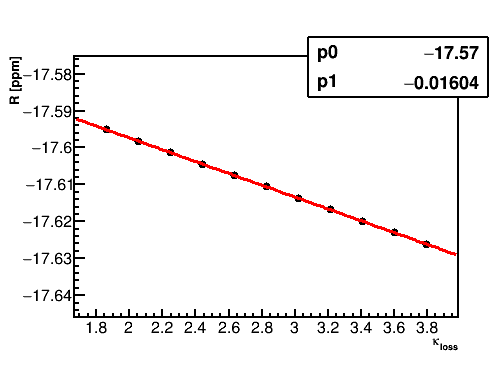
\includegraphics[width=.7\textwidth]{FullRatio_R_Vs_kappa_loss_Canv}
    \caption[Scan over fixed \K in ratio fit]{The sensitivity of \R to the fixed \K parameter. Error bars have been removed from the plot in order to show the trend more clearly. Units are in ppm, data are from the 9d dataset.}
    \label{fig:kappaLossScan}
\end{figure}


\begin{table}
\centering
\renewcommand{\arraystretch}{1.2}
\begin{tabular*}{0.75\linewidth}{@{\extracolsep{\fill}}lGcJG}
  \hline
    \multicolumn{5}{c}{\textbf{Systematic Error due to Fixed $\kappa_{loss}$}} \\
  \hline\hline
    Dataset & \multicolumn{1}{c}{$dR/d\kappa_{loss}$} & $T_{\kappa_{loss}}$ & \multicolumn{1}{c}{$\boldsymbol{\delta R}$} & \multicolumn{1}{c}{$\Delta R_{\text{(w/ - w/o)}}$} \\
  \hline
    60h & -3.06 & $8.253 \pm 0.305$ & 0.9 & -26.1 \\
    HighKick & -8.74 & $4.014 \pm 0.391$ & 3.4 & -35.1 \\
    9d & -16.04 & $2.826 \pm 0.193$ & 3.1 & -45.3 \\
    Endgame & +1.43 & $2.634 \pm 0.041$ & 0.1 & +3.8 \\
  \hline
\end{tabular*}
\caption[Systematic error due to fixed $\kappa_{loss}$]{Systematic error due to the fixed $\kappa_{loss}$ parameter in the Ratio Method fits for the Run~1 precession frequency analysis datasets. All units are in ppb except for the $T_{\kappa_{loss}}$ parameter which is unit-less. $\sigma_{\kappa_{loss}}$ comes from the T-Method fit results and scales with the number of statistics. The bold column gives the systematic errors on \R. The far right column gives the change in $R$ with the \K parameter in the fits versus without it entirely.}
\label{tab:systematicError_kappaLoss}
\end{table}
